\documentclass{article}
\usepackage[utf8]{inputenc}
\usepackage[T1]{fontenc}
\usepackage[frenchb]{babel}
\usepackage[bookmarks=true]{hyperref}
\usepackage{lmodern}
\usepackage{graphicx}


\author{Gentile Pierre, Didier-Roche François}
\date{\today}
\title{Manuel utilisateur}

\frenchbsetup{StandardLists=true}

\begin{document}

\maketitle

\newpage
\tableofcontents
\newpage

\section{Formulaires} \label{Formulaires}
Les formulaires présents dans l'application fonctionnent tous de la même manière et en deux étapes :
\begin{itemize}
  \item Remplir le formulaire en suivant les indications.
  \item Valider le formulaire via un bouton.
\end{itemize}

De ce fait, seul quelque pages de formulaires serons expliquées.
 Si vous souhaitez avoir plus d'informations sur les formulaires, voir la section \ref{S'authentifier}



\section{S'authentifier} \label{S'authentifier}
\subsection{Se connecter}
\begin{center}
  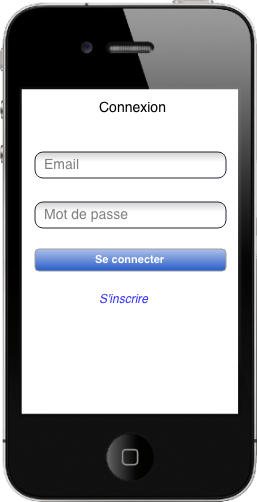
\includegraphics[width=150pt]{Interfaces/connexion}
\end{center}
Une fois l'application lancée, vous arrivez sur une page de connexion. Vous avez alors deux choix :
\begin{itemize}
  \item Vous connecter directement si vous êtes déjà inscrit en renseignant votre email et votre mot de passe et en appuyant sur le bouton "Se connecter".
  \item Vous inscrire si vous n'êtes pas déjà inscrit en appuyant sur le texte en bleu "S'inscrire" présent sous le bouton "Se connecter".
\end{itemize}


\subsection{S'inscrire}
\begin{center}
  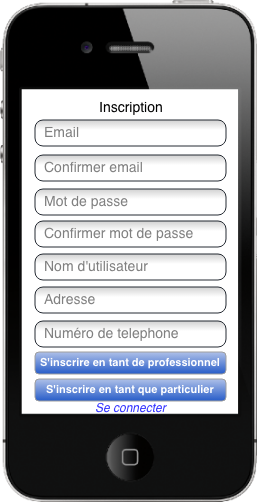
\includegraphics[width=150pt]{Interfaces/inscription}
\end{center}
Si vous choisissez de vous inscrire, vous devez renseigner tout les champs présents sur la page sur laquelle vous avez été redirigé. Vous devrez ensuite appuyer sur le bouton  :
\begin{itemize}
  \item "S'inscrire en tant que professionnel" si vous êtes un prfessionnel souhaitant proposer ses services. \item "S'inscrire en tant que particulier" si vous êtes un particulier à la recherche d'un professionnel.
\end{itemize}
Vous pouvez aussi retourner vers la page de connexion en appuyant sur le texte bleu "Se connecter" présents sous les boutons.



\subsection{Créer son entreprise}
\begin{center}
  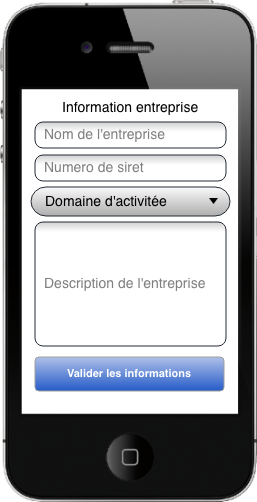
\includegraphics[width=150pt]{Interfaces/creation_entreprise}
\end{center}
Si vous avez choisissez de vous inscrire en tant que professionnel souhaitant proposer ses services, il faudra alors remplir le formulaire sur lequel vous venez d'être redirigé et appuyer sur le bouton "Valider les informations".

ATENTION ! Si vous arretez l'application à ce moment la, le formulaire que vous avez rempli à l'étape précédante n'aura pas été enregistré.

\section{Pour les particuliers (utilisateurs ne proposant pas de services)}
\subsection{Menu}
\begin{center}
  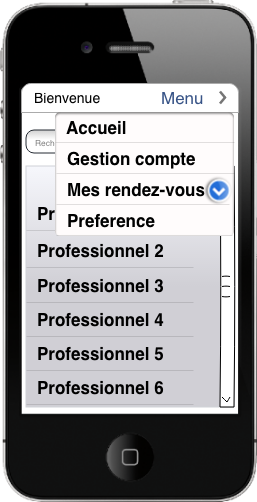
\includegraphics[width=150pt]{Interfaces/menuuser}
  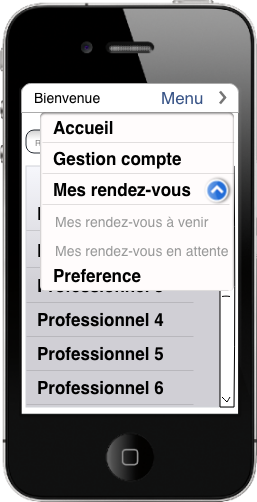
\includegraphics[width=150pt]{Interfaces/menuuserdeplier}
\end{center}
Sur toutes les pages de l'application, vous pouvez acceder à tout les fonctionnalitées que l'application vous offre en appuyant sur le texte bleu "Menu" en haut à droite de votre écran. En appuyant sur menu, l'application vous propose une liste de liens cliquables :
\begin{itemize}
  \item Accueil permetant d'aller à l'accueil.
  \item Gestion de compte permetant d'aller vers une page proposant un formulaire pour modifier une ou plusieurs informations relative à votre compte.
  \item Mes rendez-vous permetant de consulter ses rendez pris et ceux en attente de confirmation.
  \item Preferences permetant de modifier les paramètre de l'application (par exemple, les notifications).
\end{itemize}


\subsection{Accueil} \label{Accueil}
\begin{center}
  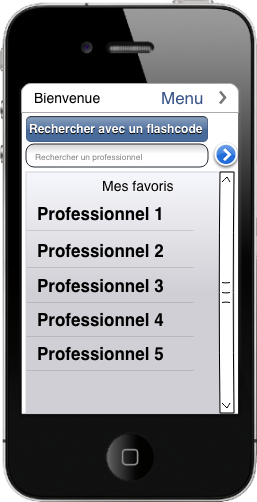
\includegraphics[width=150pt]{Interfaces/accueuil}
\end{center}
À l'accueil, vous avez plusieurs éléments utiles :
\begin{itemize}
  \item Sous la barre de menu située en haut de votre écran, un bouton "Rechercher avec un flashcode" permet de rechercher un professionnel via le flashcode (code barre) que le professionnel a indiqué. En appuyant sur ce bouton, l'application ouvrira votre appareil photo et vous devrez diriger ce dernier vers le flash code.
  \item Sous le bouton "Rechercher avec un flashcode" vous avez une barre de recherche accompagné d'un bouton afin de rechercher un professionnel par mot clé.
  \item Enfin, sous la barre de recherche, vous la liste de professionnel que vous avez ajouter en favoris qui se transforme en liste de professionnel obtenu en via votre recherche (si vous utilisez la fonction de recherche).
\end{itemize}


\subsection{Prise de rendez-vous} \label{Prise de rendez-vous}
\subsubsection{Page du professionnel}
\begin{center}
  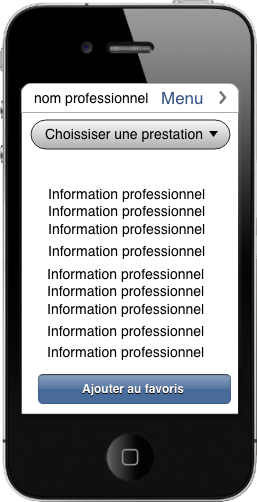
\includegraphics[width=150pt]{Interfaces/professionnel}
\end{center}
Une fois que vous avez selectionné un professionnel, l'application affiche la page suivante sur laquelle vous pouvez :

\begin{itemize}
  \item Déplier le menu deroulant "Selectionner une prestation" se trouvant sous la barre de menu en haut de votre écran.
  \item Consulter des informations relatives au professionnel et a son entreprise.
  \item Ajouter le professionnel en question au favoris.
\end{itemize}



\subsubsection{Selection de prestation}
\begin{center}
  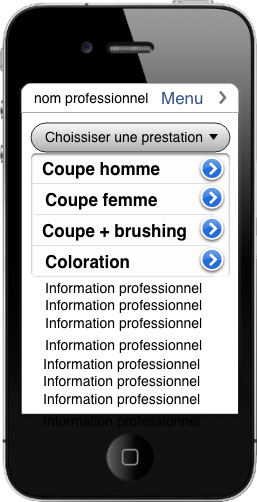
\includegraphics[width=150pt]{Interfaces/prodeplie}
\end{center}
Une fois le menu déroulant "Selectionner une prestation" déplié, vous pouvez selectionner une prestation parmis celles proposées par le professionnel en appuyant dessus.

\subsubsection{Sélection des horaires}
\begin{center}
  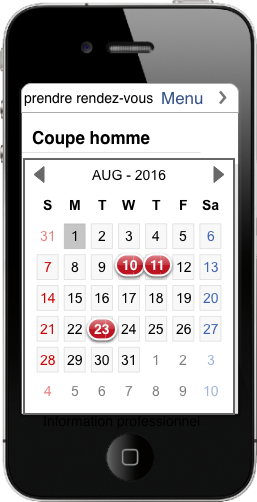
\includegraphics[width=150pt]{Interfaces/calendrier}
\end{center}
Une fois que vous avez selectionné une prestation, vous allez être redirigé vers un calendrier affichant les plage horaire qui correspondent à votre demande et qui sont disponibles en surbrillance.

\section{Pour les professionnels (utilisateur proposant des services)}
\subsection{Menu}
\begin{center}
  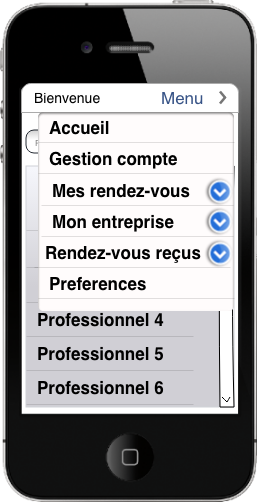
\includegraphics[width=150pt]{Interfaces/menupro}

\end{center}
Sur toutes les pages de l'application, vous pouvez acceder à tout les fonctionnalitées que l'application vous offre en appuyant sur le texte bleu "Menu" en haut à droite de votre écran. En appuyant sur menu, l'application vous propose une liste de liens cliquables :
\begin{itemize}
  \item Accueil permetant d'aller à l'accueil.
  \item Gestion de compte permetant d'aller vers une page proposant un formulaire pour modifier une ou plusieurs informations relative à votre compte.
  \item Mes rendez-vous permetant de consulter ses rendez pris et ceux en attente de confirmation.
  \item Mon entreprise permetant de modifier des informations relative à votre entreprise, créer de nouvelles prestations ou modifier les disponibilitées du calendrier.
  \item Rendez-vous reçus permetant de consulter ses demande de rendez-vous en attente de confirmation et ses rendez-vous déjà accepté à venir.
  \item Preferences permetant de modifier les paramètre de l'application (par exemple, les notifications).
\end{itemize}

\subsection{Accueil}
 Voir section \ref{Accueil}
\subsection{Prise de rendez-vous}
 Voir section \ref{Prise de rendez-vous}











\end{document}
